% \iffalse
\let\negmedspace\undefined
\let\negthickspace\undefined
\documentclass[journal,12pt,twocolumn]{IEEEtran}
\usepackage{cite}
\usepackage{amsmath,amssymb,amsfonts,amsthm}
\usepackage{algorithmic}
\usepackage{graphicx}
\usepackage{textcomp}
\usepackage{xcolor}
\usepackage{txfonts}
\usepackage{listings}
\usepackage{enumitem}
\usepackage{mathtools}
\usepackage{gensymb}
\usepackage{comment}
\usepackage[breaklinks=true]{hyperref}
\usepackage{tkz-euclide} 
\usepackage{listings}
\usepackage{gvv}                                        
\def\inputGnumericTable{}                                 
\usepackage[latin1]{inputenc}                                
\usepackage{color}                                            
\usepackage{array}                                            
\usepackage{longtable}                                       
\usepackage{calc}                                             
\usepackage{multirow}                                         
\usepackage{hhline}                                           
\usepackage{ifthen}                                           
\usepackage{lscape}
\usepackage{placeins}

\newtheorem{theorem}{Theorem}[section]
\newtheorem{problem}{Problem}
\newtheorem{proposition}{Proposition}[section]
\newtheorem{lemma}{Lemma}[section]
\newtheorem{corollary}[theorem]{Corollary}
\newtheorem{example}{Example}[section]
\newtheorem{definition}[problem]{Definition}
\newcommand{\BEQA}{\begin{eqnarray}}
\newcommand{\EEQA}{\end{eqnarray}}
\newcommand{\define}{\stackrel{\triangle}{=}}
\theoremstyle{remark}
\newtheorem{rem}{Remark}

\begin{document}

\bibliographystyle{IEEEtran}
\vspace{3cm}

\Large\title{NCERT Question 10.5.2.5}
\large\author{EE23BTECH11032 - Kaustubh Parag Khachane $^{*}$% <-this % stops a space
}
\maketitle
\newpage
\bigskip

\renewcommand{\thefigure}{\theenumi}
\renewcommand{\thetable}{\theenumi}
\large\textbf{Question 10.5.2.5} : \normalsize Find the number of terms in each of the following APs : 

(i) 7, 13, 19, ... 205

(ii) 18, 15\(\frac{1}{2}\), 13, ... -47

\vspace{4mm} 

\large\textbf{Solution} :\normalsize

\vspace{4mm}

\textbf{(i)} The \(n^{th}\) term of the Arithmetic progression is given as a + (n-1)d where a is the first term and d is the common difference.

The common difference of the AP is given by the difference between successive terms.

\vspace{4mm}

Common difference (d) = 13 - 7 = 6

First term (a) = 7

\vspace{4mm}

If 205 is the \(n{th}\) term of the series, we have :
\begin{align}
&205 = 7 + (n-1)6\\ 
\implies&  198 = (n-1)6\\
\implies&  33 = n-1\\
\implies& n = 34
\end{align}

\large\textbf{Answer} : \normalsize There are 34 elements in the series.

\vspace{4mm}

\textbf{(ii)} The \(n^{th}\) term of the Arithmetic progression is given as a + (n-1)*d where a is the first term and d is the common difference.

The common difference of the AP is given by the difference between successive terms.

\vspace{4mm}

Common difference (d) = 15\(\frac{1}{2}\) - 18 = -2\(\frac{1}{2}\)

First term (a) = 18

\vspace{4mm}

If -47 is the \(n{th}\) term of the series, we have :
\begin{align}
&-47 = 18 + (n-1)\left(-2\left(\frac{1}{2}\right)\right)\\ 
\implies& -65 = (n-1)\left(-2\left(\frac{1}{2}\right)\right)\\
\implies& 26 = n-1\\
\implies& n = 27
\end{align} 

\large\textbf{Answer} : \normalsize There are 27 elements in the series.

\vspace{10mm}

\large\textbf{Question} : \normalsize Express the $n^{th}$ term in each case as x(n) and find its z transform.

\vspace{4mm}

\large\textbf{Solution} : \normalsize

\vspace{4mm}

\textbf{(i)} The \(n^{th}\) term of the Arithmetic progression ($T_{n}$) is given as a + (n-1)d where a is the first term and d is the common difference.

\begin{align}
\therefore T_{n} = 7 + (n-1)6 \\
x(n) = 7 + (n-1)6
\end{align}
The Z transformation for x[n] is given by :

\begin{align}
    X(z) =\left[ \sum_{n=-\infty}^{\infty}x[n]z^{-n}\right]
\end{align}

However, x[n] cannot be summed from $-\infty$ to zero as the number of terms cannot be negative due to which the $n^{th}$ will not be defined for this range of n.\\
So, we will modify x[n] by multiplying it with unit step function(u(n)) so we have the value as zero for n$<$1.

\begin{align}
&x(n) = \left(7 + (n-1)6\right)u(n) \\
     x\brak{n} & = \begin{cases}
        0 & \text{for } n < 1 \\
        7 + (n-1)6 & \text{for } n \geq 1
    \end{cases}
\end{align}
Now, using the above function in equation (11):

\begin{align}
X(z) &= \sum_{n=1}^{\infty}x[n]z^{-n}\\
 &= \sum_{n=1}^{\infty}(a+(n-1)d)z^{-n} \\
 &=  \left[\sum_{n=1}^{\infty}az^{-n} \right] + \left[ \sum_{n=1}^{\infty}(nd)z^{-n} \right] - \left[ \sum_{n=1}^{\infty}dz^{-n} \right]
 \end{align}
\begin{align}
 &=  \left[\sum_{n=1}^{\infty}7z^{-n} \right] + \left[ \sum_{n=1}^{\infty}(6n)z^{-n} \right] - \left[ \sum_{n=1}^{\infty}6z^{-n} \right]\\
 &=  \left[\sum_{n=1}^{\infty}z^{-n} \right] + \left[ \sum_{n=1}^{\infty}(6n)z^{-n} \right]\\
 &= \frac{1}{z-1} + 6\left[ \sum_{n=1}^{\infty}(n)z^{-n} \right]
\end{align}
Calculating the integral in the above expression :\\
\begin{align}
&S =  \left[\sum_{n=1}^{\infty}(n)z^{-n}\right ]\\ 
&S = z^{-1} + 2z^{-2} + 3z^{-3} + ...\\
&Sz^{-1} = z^{-2} + 2z^{-3} + 3z{-4} + ... 
\end{align}
Subtracting (22) and (21) \\
\begin{align}
S(1-z^{-1}) &= z^{-1} + z^{-2} + z^{-3} + ... \\
 &= \frac{1}{(z-1)(1-z^{-1})}\\
 &= \frac{1}{z-2+z^{-1}}\\
\therefore S &= \frac{z}{(z-1)^2}
\end{align}
Using equations (26) and (19) :\\
\begin{align}
X(z) &= \frac{1}{z-1} + \frac{6z}{(z-1)^2}\\
 &= \frac{7z-1}{(z-1)^2}
\end{align}
\large\textbf{Answer} : \normalsize The z transformation for x(n) where x(n) is the $n^{th}$ term of the AP is $\frac{7z-1}{(z-1)^2}$.
\vspace{4mm}

\textbf{(ii)} The \(n^{th}\) term of the Arithmetic progression ($T_{n}$) is given as a + (n-1)d where a is the first term and d is the common difference.

$\therefore T_{n} = 18 + (n-1)\left(-2\frac{1}{2}\right) $

$x(n) = 18 + (n-1)\left(-2\frac{1}{2}\right)$

The Z transformation for x[n] is given by : \\
\begin{align}
X(z) =\left[ \sum_{n=-\infty}^{\infty}x[n]z^{-n}\right]
\end{align}
\\
\vspace{15mm}
However, x[n] cannot be summed from $-\infty$ to zero as the number of terms cannot be negative due to which the $n^{th}$ will not be defined for this range of n.\\
So, we will modify x[n] by multiplying it with unit step function(u(n)) so we have the value as zero for n$<$1.
\begin{align}
&x(n) = \left(18 + (n-1)\left(-2\frac{1}{2}\right)\right)u(n) \\
     x\brak{n} & = \begin{cases}
        0 & \text{for } n < 1 \\
        18 +(n-1)\left(-2\frac{1}{2}\right) & \text{for } n \geq 1
    \end{cases}
\end{align}
\begin{align}
X(z) &= \sum_{n=1}^{\infty}x[n]z^{-n}\\
 &= \sum_{n=1}^{\infty}(a+(n-1)d)z^{-n} \\
 &=  \left[\sum_{n=1}^{\infty}az^{-n} \right] + \left[ \sum_{n=1}^{\infty}(nd)z^{-n} \right] - \left[ \sum_{n=1}^{\infty}dz^{-n} \right]\\
 &=  \left[\sum_{n=1}^{\infty}18z^{-n} \right] + \left[ \sum_{n=1}^{\infty}(n)\left(-2\frac{1}{2}\right)z^{-n} \right] - \left[ \sum_{n=1}^{\infty}\left(-2\frac{1}{2}\right)z^{-n} \right]\\
 &=  \left[\sum_{n=1}^{\infty}\left(20\frac{1}{2}\right)z^{-n} \right] - \left[ \sum_{n=1}^{\infty}\left(n\left(2\frac{1}{2}\right)\right)z^{-n} \right]\\
 &= \left(20\frac{1}{2}\right)\left[\sum_{n=1}^{\infty}z^{-n} \right] - \left[ \sum_{n=1}^{\infty}\left(n\left(2\frac{1}{2}\right)\right)z^{-n} \right]\\
 &= \left(20\frac{1}{2}\right)\frac{1}{z-1} - \left(2\frac{1}{2}\right)\left[ \sum_{n=1}^{\infty}(n)z^{-n} \right]\\
 &= \left(20\frac{1}{2}\right)\frac{1}{z-1} - \left(2\frac{1}{2}\right)S
\end{align}

Using equation (26) and (39) : \\
\begin{align}
X(z) &=  \left(20\frac{1}{2}\right)\frac{1}{z-1} - \left(2\frac{1}{2}\right)\frac{z}{(z-1)^2}\\
&= \frac{18z - \left(20\frac{1}{2}\right)}{(z-1)^2}
\end{align}
\large\textbf{Answer} : \normalsize The z transformation for x(n) where x(n) is the $n^{th}$ term of the AP is $\frac{18z - \left(20\frac{1}{2}\right)}{(z-1)^2}$.

\newpage

\large\textbf{Question} : \normalsize Plot the graph of x(n) and find the ROC of X(z) in each case.

\large\textbf{Solution} :\\
\large\textbf{(i)} \normalsize The graph of x(n) is :
\begin{figure}[h]
    \begin{center}
    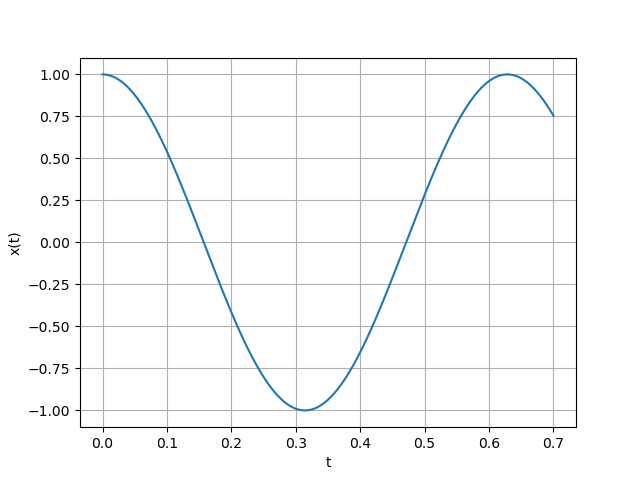
\includegraphics[width = 9cm]{Figure_1}
    Fig. 0. Plot of x(n) \\
    \end{center}
\end{figure}

The ROC (Region of Convergence) of x(n) is defined as the range of values of z for which X(z) will converge where X(z) is the z transform of x(n).\\
\begin{align}
   \left|X(z)\right| = \sum_{n = -\infty}^{\infty}\left|x(n)z^{-n}\right| < \infty
\end{align}

By equation (18) :\\
\begin{align}
X(z) &=  \left[\sum_{n=1}^{\infty}z^{-n} \right] + 6\left[ \sum_{n=1}^{\infty}(n)z^{-n} \right]
\end{align}
The sum $ \left[\sum_{n=1}^{\infty}z^{-n} \right]$ will converge only if z is not zero and $\left|z^{-1}\right| < 1$ (or $|z| > 1$) as it is forming an infinite GP with common difference $z^{-1}$.\\

Observe the second part of the equation (43)(or 18) is 6S which was calculated using equation (23) : \\
\begin{align}
    S(1-z^{-1}) &= z^{-1} + z^{-2} + z^{-3} + ... 
\end{align}
The sum S will converge only if z is not 0 and $\left|z^{-1}\right| < 1$ as again we obtain an infinite GP with common difference $z^{-1}$.For both the parts of the equation (45), the ROC is same.

\vspace{4mm}

\large\textbf{Answer} : \normalsize The ROC of X(z) is  $|z| > 1$

\vspace{8mm}

\large\textbf{(ii)} \normalsize The graph of x(n) is :

\vspace{4mm}

\begin{figure}[!h]
    \begin{center}
    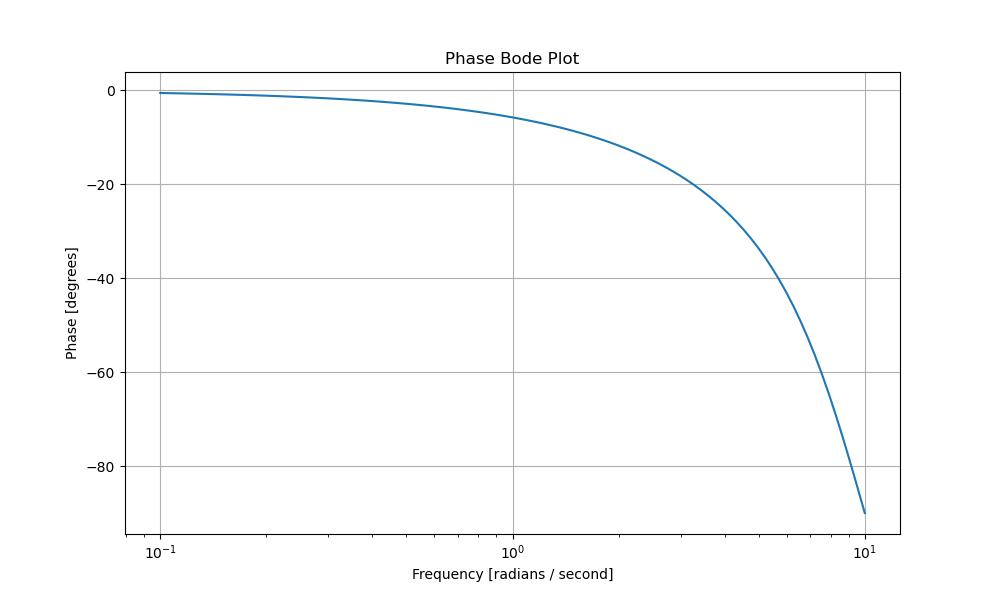
\includegraphics[width = 9cm]{Figure_2}
    Fig. 1. Plot of x(n) \\
    \end{center}
\end{figure}

\FloatBarrier

The ROC (Region of Convergence) of x(n) is defined as the range of values of z for which X(z) will converge where X(z) is the z transform of x(n).\\
\begin{align}
   \left|X(z)\right| = \sum_{n = -\infty}^{\infty}\left|x(n)z^{-n}\right| < \infty
\end{align}

By equation (37) :\\
\begin{align}
X(z) = \left(20\frac{1}{2}\right)\left[\sum_{n=1}^{\infty}z^{-n} \right] - \left(2\frac{1}{2}\right)\left[ \sum_{n=1}^{\infty}\left(n\right)z^{-n} \right]
\end{align}
The sum $ \left[\sum_{n=1}^{\infty}z^{-n} \right]$ will converge only if z is not zero and $\left|z^{-1}\right| < 1$ ( or $|z| > 1$) as it is forming an infinite GP with common difference $z^{-1}$.\\

Observe the second part of the equation (46)(or 37) is $-2\frac{1}{2}$S which was calculated using equation (23) : \\
\begin{align}
    S(1-z^{-1}) &= z^{-1} + z^{-2} + z^{-3} + ... 
\end{align}
The sum S will converge only if z is not 0 and $\left|z\right| < 1$ as again we obtain an infinite GP with common difference $z^{-1}$.For both the parts of the equation (47), the ROC is same.

\vspace{4mm}

\large\textbf{Answer} : \normalsize The ROC of X(z) is  $|z| > 1$

\end{document}
